% Research article (deliverable 2) — one-claim conference-style paper.
% Build: latexmk -pdf article.tex
% THE CLAIM: distillation saturates at 0.6B, and what fine-tuning actually buys
% an on-device traffic controller is AUTHORSHIP (audit-meaningful control), not delay.
\documentclass[conference]{IEEEtran}
\usepackage[T1]{fontenc}
\usepackage[utf8]{inputenc}
\usepackage{graphicx}
\usepackage{tikz}
\usepackage{pgfplots}
\pgfplotsset{compat=1.18}
\usetikzlibrary{arrows.meta,positioning}
\definecolor{nbblue}{HTML}{1F4E79}
\definecolor{nbteal}{HTML}{2E8B8B}
\definecolor{nbred}{HTML}{B83227}
\definecolor{nbgrey}{HTML}{555555}
\definecolor{nbband}{HTML}{EAF0F6}
\usepackage{booktabs}
\usepackage{amsmath}
\usepackage{xcolor}
\usepackage[hidelinks]{hyperref}
\usepackage{cite}

\newcommand{\todo}[1]{{\color{red}\footnotesize [TODO: #1]}}

\begin{document}

\title{Authorship, Not Delay: What Frontier Distillation Buys an On-Device
Small-Language-Model Traffic Controller}

\author{\IEEEauthorblockN{Ebenezer Veeraraju}
\IEEEauthorblockA{Dept.\ of Computer Science, University College London\\
ebenezer.veeraraju.24@ucl.ac.uk}
\and
\IEEEauthorblockN{Akin Delibasi}
\IEEEauthorblockA{University College London\\
a.delibasi@ucl.ac.uk}
\and
\IEEEauthorblockN{Lee Stott}
\IEEEauthorblockA{Microsoft\\
leestott@microsoft.com}}

\maketitle

\begin{abstract}
Large-language-model traffic signal controllers are evaluated in the cloud,
but junctions run at the edge, and after an accident someone must prove
which controller did what. We present, to our knowledge, the first traffic
signal controller fine-tuned and served entirely on-device: a
QLoRA-distilled small language model (SLM) compiled to int4 ONNX and served by Microsoft Foundry
Local on a 6\,GB consumer GPU, controlling measured London topologies in SUMO
behind a MaxPressure safety shield with a tamper-evident, Ed25519 hash-chained
decision audit. Distilling a frontier teacher lifts held-out decision accuracy
from 55--69\% to 97--99\% and \emph{saturates by 0.6B parameters}: a 3.8B
student is statistically indistinguishable from a 0.6B one, within
$\pm0.38\%$ of closed-loop delay. Whether accuracy becomes delay depends on
whether the test network can express it: on saturated maps, over 30
training-disjoint seeds, no arm significantly beats a fixed-time floor.
But on the same grid demand-calibrated so that traffic actually flows,
the distilled controller beats that floor by 8.8\% while the stock one
loses to it by 11.9\%, an \emph{18.3\% head-to-head improvement on 30 of
30 seeds} ($p{=}2.0{\times}10^{-21}$) that gridlock had been masking. The same
calibration does not reproduce that effect on a second network, and we
report that failed replication. Everywhere,
fine-tuning raises the SLM's share of logged decision ticks from
0.39--0.62 to 0.56--0.77, because the distilled policy trips the
anti-starvation floor far less often, while its divergence from
MaxPressure falls from 0.46--0.60 to 0.04--0.17. We argue authorship is
the property an audit needs: an audit of the stock deployment could
attribute two decisions in five to the learned component, against four in
seven after distillation, a deterministic timer authoring the
rest. We state the deflationary reading, that distillation partly
taught imitation of the classical reference, and bound it with the
evidence.
\end{abstract}

\section{Introduction}\label{sec:intro}
LLM-based traffic signal control has moved quickly from prompting to
fine-tuning \cite{lai2023llmlight,wang2025trafficr1,curalight2026}, but the
deployment story has not moved with it: every published controller is
evaluated against a cloud endpoint, while the signal cabinet at a junction is
an edge device with tight memory, no service-level guarantee to the cloud, and
a statutory duty, unique among LLM application domains, to explain itself
after a collision. A junction controller that cannot be audited is not
deployable regardless of its delay numbers.

This paper asks what fine-tuning actually contributes to an SLM traffic
controller that runs \emph{entirely} on-device under a classical safety
shield. We fine-tune with QLoRA \cite{dettmers2023qlora} on decisions
distilled from a frontier teacher, compile to int4 ONNX, and serve with
Microsoft Foundry Local on a consumer RTX~2060 (6\,GB) of roughly
signal-cabinet class. Control runs in SUMO on topologies built from
measured London data (Euston A501 at DfT-measured peak-hour magnitude, a Bloomsbury grid,
Old Street junction), with a MaxPressure \cite{varaiya2013maxpressure} shield
and anti-starvation floor between the model and the lights, and every decision
bound into a hash-chained, signed audit record.

Contributions:
\begin{itemize}
\item \textbf{A documented QLoRA$\to$int4$\to$Foundry-Local chain.} To our
knowledge the first published recipe for serving a custom fine-tuned model
through Foundry Local, including the registration and execution-provider
steps the toolchain does not document, with equal aggregate holdout
accuracy between CPU and WebGPU serving.
\item \textbf{A scale-saturation result.} Frontier distillation lifts a
0.6B student to 97--99\% holdout agreement with the teacher, and a 3.8B
student lands on the same numbers. For this task class, the bottleneck is
not capability but the distillation ceiling.
\item \textbf{A large, seed-unanimous effect and the measurement condition
needed to see it.} Distillation is worth under two points on an
oversaturated grid, but 18.3\% on 30 of 30 seeds once that grid is
calibrated to flow.
Oversaturated test networks compress controller effect sizes, which has
implications beyond this study.
\item \textbf{The authorship finding.} Where delay effects are compressed,
accuracy still decouples from delay, but fine-tuning raises the model's
share of logged decision ticks by up to 17 points and cuts its divergence from
the classical reference four-fold. We define authored share on the
decision-tick denominator, the quantity a decision audit needs, and separate
it from proposal acceptance.
\item \textbf{Honest nulls with mechanism.} We report the closed-loop
nulls where they occur, the guard metrics that decide which delay numbers
are comparable, and the failure tail with its audit-chain forensics.
\end{itemize}

\section{Related work}\label{sec:related}
LLMLight \cite{lai2023llmlight} distils GPT-4 rationales into LoRA-tuned
students down to 0.5B and remains the closest prior work, but evaluates on
CityFlow grids against cloud-served checkpoints. Traffic-R1
\cite{wang2025trafficr1} applies R1-style RL to a 3B model and CuraLight
\cite{curalight2026} is the one fine-tuning work on SUMO. DGLight
\cite{dglight2026} tunes an 8B model with GRPO and, usefully for calibration,
reports the \emph{entire} LLM-vs-MaxPressure gap at 1--2\%. iLLM-TSC
\cite{pang2024illmtsc} inverts our topology by letting an RL agent propose
and a cloud LLM veto, which prices the veto path at cloud latency and
availability. Our deterministic local verifier costs $O(\text{phases})$ per
decision. None of these serve on-device, none pair control with a
tamper-evident audit, and none evaluate on measured UK topologies. Our
shield is deliberately weaker than correct-by-construction shielding
\cite{alshiekh2018shield}: it composes preemptive action masking
\cite{huang2020masking}, post-posed default substitution, and an
anti-starvation runtime monitor, and we discuss what a formal upgrade would
require.

\section{System and method}\label{sec:method}
\begin{figure*}[t]
\centering
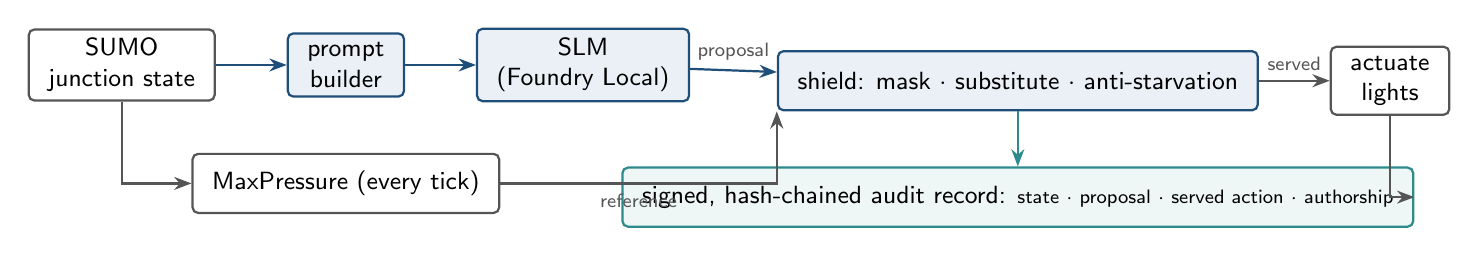
\begin{tikzpicture}[
  node distance=5mm and 9mm,
  box/.style={draw=nbblue, thick, rounded corners=2pt, fill=nbband,
    font=\sffamily\small, minimum height=7.5mm, inner xsep=2.5mm, align=center},
  det/.style={box, draw=nbgrey, fill=white},
  aud/.style={box, draw=nbteal, fill=nbteal!8},
  arr/.style={-{Stealth[length=2.2mm]}, thick, nbblue},
  darr/.style={-{Stealth[length=2.2mm]}, thick, nbgrey},
  lab/.style={font=\sffamily\scriptsize, text=nbgrey}]
\node[det] (sumo) {SUMO\\junction state};
\node[box, right=of sumo] (prompt) {prompt\\builder};
\node[box, right=of prompt] (slm) {SLM\\(Foundry Local)};
\node[box, right=of slm, yshift=-2mm, xshift=2mm] (shield)
  {shield: mask $\cdot$ substitute $\cdot$ anti-starvation};
\node[det, below=of prompt, yshift=-2mm] (mp) {MaxPressure (every tick)};
\node[det, right=of shield] (act) {actuate\\lights};
\node[aud, below=of shield, yshift=-2mm] (audit)
  {signed, hash-chained audit record:
  \scriptsize state $\cdot$ proposal $\cdot$ served action $\cdot$ authorship};
\draw[arr] (sumo) -- (prompt);
\draw[arr] (prompt) -- (slm);
\draw[arr] (slm) -- node[lab, above]{proposal} (shield);
\draw[darr] (sumo.south) |- (mp.west);
\draw[darr] (mp.east) -| node[lab, below, pos=0.25]{reference} (shield.south west);
\draw[darr] (shield) -- node[lab, above]{served} (act);
\draw[darr] (act.south) |- (audit.east);
\draw[arr, nbteal] (shield.south) -- (audit.north);
\end{tikzpicture}
\caption{The junction control loop. The deterministic path (grey) is
complete without the SLM. The learned proposer (blue) attaches to it, and
every served decision lands in the signed audit chain (teal).}
\label{fig:arch}
\end{figure*}

\subsection{Control loop and shield}
Each junction is polled on a fixed decision interval ($\approx$10\,s
simulated). The SLM receives junction state in one of four prompt formats of
increasing privilege: \emph{myopic} (per-phase halting counts),
\emph{sota} (delay-aware), \emph{prediction} (arrival forecasts),
\emph{coordination} (neighbour notes). It must return exactly
\texttt{\{"phase": N\}}. The shield masks the menu to conflict-free phases,
substitutes the MaxPressure phase when output is invalid, and enforces a
minimum-service floor. We define \textbf{divergence rate} as the fraction of
SLM-authored decisions whose served phase differs from what MaxPressure would
have chosen, and \textbf{authored share} as the fraction of logged decision
ticks whose served phase originated with the SLM. Divergence is measured among
decisions the SLM did author, so it describes how far the learned policy
departs from the classical reference when it is in control. The harness field
carrying it is named \texttt{override\_rate} for historical reasons, which is
a misnomer because the shield's substitution path fires on 0.5\% of
decisions in the one cell where it fires at all. These are interference metrics in the sense of the shielding
literature, not veto counts.

\subsection{Audit}
Every logged decision emits a record (halting-queue state, model proposal,
shield proposal, served action, serving authorship, override flag) that is
Ed25519-signed per junction and hash-chained into a single append-only chain
per run, with model identity and latency recorded at run level, and chains
verify end-to-end after each run. After a
simulated collision the system assembles a cited evidence pack against a UK
traffic-law knowledge base. That pack is deliberately not a verdict,
following the legal-hallucination risk analysis of \cite{dahl2024legal}.

\subsection{Distillation and training}
We sample 48{,}137 junction states from eight training-reserved seeds, label
them with a frontier teacher (cross-audited against a second: $\sim$98\%
agreement), and render 59{,}533 examples in four formats with
family-correct templates and completion-only loss. A hash-based split
freezes a 5{,}580-example holdout pre-training. Students: Qwen3-0.6B and
Phi-4-mini (3.8B), QLoRA $r{=}16$ NF4, merged to bf16, compiled to int4 ONNX
(RTN weight-only) via the onnxruntime-genai builder, registered in Foundry
Local. The 0.6B trains on the serving GPU in 13.5\,h, the 3.8B on an
RTX~4090 in 2.3\,h. Stock controls are the \emph{same} base model on the
\emph{identical} int4 pipeline. Two 0.6B fine-tunes exist:
Table~\ref{tab:offline}'s four-format generalist and the sota-only ft1 in
all closed-loop sweeps. On ft1, CPU and WebGPU score identically in aggregate on the
holdout (97.42\% both; per-item outputs were not retained, so this is
equal accuracy, not demonstrated output identity), so sweeps run
GPU-served.

\subsection{Closed-loop protocol}
Closed-loop cells pair the controller against MaxPressure in loop and a
fixed-time floor on the same seeds, disjoint from the eight training-state
seeds. Because the route files are static, with fixed vehicle identities
and departure times, and the SUMO seed varies microscopic car-following and
lane-change randomness rather than the demand, that disjointness narrows
trajectory-level leakage without closing it: head-to-head arm comparisons
are unaffected, but generalisation beyond the trained demand is not
established. Per topology and arm: $n{=}30$ seeds, paired $t$ on mean network
delay.

\section{Evaluation}\label{sec:eval}

\subsection{Offline: distillation saturates at 0.6B}
Table~\ref{tab:offline} shows holdout agreement with the frozen teacher
labels, stock vs fine-tuned, both students, int4-as-served.

\begin{table}[t]
\caption{Holdout accuracy (\%) vs frontier teacher, int4-as-served.
Strict-JSON compliance in parentheses where below 100\%.}
\label{tab:offline}
\centering
\small
\begin{tabular}{lcccc}
\toprule
 & myopic & sota & prediction & coordination \\
\midrule
Qwen3-0.6B stock & 45.6 & 55.1 (93.4) & 63.3 & 69.3 \\
Qwen3-0.6B ft    & 87.9 & 97.7 & 97.6 & 99.0 \\
Phi-4-mini stock & 87.5 & 59.0 & 86.0 & 87.0 \\
Phi-4-mini ft    & 88.7 & 97.1 & 97.4 & 99.3 \\
Phi-4-mini LOTO  & 88.3 & 96.8 & 97.4 & 99.1 \\
\bottomrule
\end{tabular}
\end{table}

Three observations. First, the two fine-tuned students are statistically
indistinguishable despite a $6\times$ parameter gap, and both sit at the
teacher-agreement ceiling (the myopic ceiling is intrinsically lower: the
teacher saw state the myopic prompt hides). Distillation \emph{saturates}
this task at 0.6B. Second, where the gain lands depends on the base model:
the 0.6B is lifted everywhere (+30 to +43 points), but stock Phi-4-mini is
100\% format-compliant and 86--88\% accurate on three formats, so it gains
substantially only on the delay-aware format (+38.1 points). For a capable
base model, fine-tuning raises decision quality, not format discipline. Third,
a leave-out-topology student (LOTO, trained
with no Old Street states) matches the generalist on every format, which is
evidence against topology memorisation \emph{in aggregate} rather than
parity on the withheld layout: the holdout is scored whole with no topology
filter, and Old Street is 4.2\% of the sota rows and 0.4\% of coordination,
so this bounds a held-out-topology deficit near 7 points rather than
measuring one. Per-topology accuracy was not retained.

\subsection{Closed-loop: delay decouples from accuracy}
Table~\ref{tab:closedloop} reports the Qwen3-0.6B closed-loop sweep
(fine-tuned ft1 vs identically-compiled stock ft0), paired per-seed against
both classical comparators, which disagree in sign on one of three maps.

\begin{table}[t]
\caption{Closed-loop mean network delay against both classical
comparators ($n{=}30$ disjoint seeds). Bold = significant at $p<.05$ on
the fixed-time comparison.}
\label{tab:closedloop}
\centering
\small
\begin{tabular}{llrrr}
\toprule
Topology & Arm & vs fixed-time & vs MaxPr. & override \\
\midrule
Euston peak-hour & ft & $+15.5\%$ & $-3.9\%$ & 0.12 \\
                 & stock & $+7.6\%$ & $-6.2\%$ & 0.46 \\
Bloomsbury grid  & ft & $+0.8\%$ & $+0.7\%$ & 0.17 \\
                 & stock & $\mathbf{+2.8\%}$ & $+2.6\%$ & 0.46 \\
Old Street       & ft & $\mathbf{-11.6\%}$ & $-3.1\%$ & 0.11 \\
                 & stock & $\mathbf{-9.7\%}$ & $-1.1\%$ & 0.60 \\
\midrule
Pooled ($n{=}90$) & ft & $+1.6\%$ & $-2.1\%$ & n/a \\
\bottomrule
\end{tabular}
\end{table}

The comparator decides the outcome: against fixed-time every arm beats it
on Old Street and nowhere else, while against MaxPressure only stock on the
congested grid differs. What is invariant: a $+42$-point offline accuracy
gain buys no consistent delay change, and the one protective effect is
real. Stock harms the congested grid, $+2.8\%$ vs fixed-time
($p{=}.005$) and $-1.8\%$ head-to-head ($p{=}.022$).
A Phi-4-mini confirmation arm (same 90 cells) lands arm-for-arm on the
0.6B student's numbers, so saturation holds closed-loop as well.

The decisive evidence came from asking why the effects were so small.
Throughput guards showed the Bloomsbury map never cleared: under 15\% of
vehicles completed and $\sim$120 per run were teleported out of deadlock,
and tripling the horizon made it worse (830 teleports), proving demand
above capacity. We therefore demand-calibrated the map to 40\% (87.6\%
completion, zero teleports, matching an earlier calibration of Old
Street), kept the oversaturated cells, and re-ran all three arms on the
identical 30 seeds. \textbf{On the network that flows, the stock model
degrades delay by 11.9\%} [+10.0, +13.8] against the fixed-time floor
while both fine-tuned students \textbf{beat that floor by 8.8\%} (0.6B:
$-8.8\%$ [$-9.4, -8.2$] and 3.8B: $-8.8\%$ [$-9.3, -8.3$]), drawing level
with MaxPressure to within $0.03\%$. Head-to-head,
\textbf{fine-tuning is worth $-18.3\%$} [$-19.8, -16.8$],
$p{=}2.0{\times}10^{-21}$, \textbf{winning 30 of 30 seeds}, reproduced
identically by the 3.8B student ($-18.3\%$, 30/30,
$p{=}8.2{\times}10^{-22}$). The gridlock had been masking the
effect: a deadlocked network has a ceiling on further degradation, and
teleports truncate exactly the worst journeys, compressing good and bad
control toward the same mean. The methodological corollary generalises:
oversaturated test networks systematically understate controller effect
sizes, and since the field evaluates mostly on synthetic grids under
demand rarely reported in clearance terms, with its own calibration for
the whole LLM-vs-MaxPressure gap at 1 to 2\% \cite{dglight2026}, published
effect sizes may be compressed by the same cause. Applying the same guard
rule to the arterial corridor does not reproduce the effect. Calibrated
Euston clears (completion rises from 45--51\% to 68--74\%), but the
fine-tuned arm is still $+8.5\%$ against the fixed-time floor
($p{=}.12$) and the head-to-head gain shrinks to $-3.7\%$ in the mean,
not significant ($p{=}.63$), with a $-7.4\%$ median on 23 of 30 seeds. We
report that failure because the rule was applied where it could damage
the claim, and it did. The title claim is
therefore scoped, not withdrawn: authorship is what fine-tuning moves
everywhere, and delay only where the network can clear, and not on every
network that can.

Forensics on the failure tail qualifies this. Of 270 closed-loop cells, 14
are catastrophic ($\ge{+}20\%$ delay). All their audit chains verify, and
the catastrophic seeds are baseline-easy or median realisations, so the
failures are a controller property rather than seed hardness. The two
fine-tuned students converge at the trajectory level on a substantial
minority of cells: across 90 shared cells they produce bit-identical mean
delay on nine and agree within 0.5 points on 25 more, differing on the
remaining 56. The identical cells are separate runs whose wall-clock and median
latency differ substantially but which serve the same phase sequence.
Four of the five catastrophic fine-tuned cells fall inside this converged
subset, which restates the convergence by construction rather than
explaining it; the independent evidence is the decision-level agreement
above. Two students of
different architecture and $6\times$ different scale reproducing each
other's control trajectory exactly on a tenth of cells, and to within 0.5
points on a quarter more, is a behavioural
counterpart to the offline saturation, though partial convergence is also
consistent with both defaulting alike on easier cells. We did not separate
those explanations.

\subsection{Authorship: what fine-tuning actually moves}
Three quantities must be kept apart, and conflating them is easy: the SLM's
share of \emph{all} logged decision ticks (authorship), the fraction of its
valid proposals that survive to actuation (acceptance), and the fraction of
its own decisions differing from MaxPressure (divergence). Fine-tuning moves
all three by different amounts. On the three uncalibrated maps authorship
rises from 0.39--0.62 to 0.56--0.70, acceptance from 0.54--0.68 to
0.70--0.90, and divergence falls from 0.46--0.60 to 0.11--0.17. On the
calibrated grid the same contrast is sharper still, authorship 0.59 to
0.76--0.77 and divergence 0.56 to 0.04, which is where the 0.77 upper bound and
0.04 lower bound quoted in the abstract come from. The shield's
substitution path is inert on every cell but one (0.0\% of decisions,
0.5\% for the fine-tuned arm on Bloomsbury) because both stock and
fine-tuned models emit well-formed proposals essentially always, so the
competition for authorship is not the shield but the anti-starvation
floor, which still forces 23--44\% of decision ticks even under the best
fine-tuned arm.
This is the paper's claim: for a shielded, audited edge controller, the
deployable product of distillation is \textbf{authorship}. An accident audit
over the stock Old Street deployment could attribute only 39\% of decision ticks
to the learned component, but over the distilled deployment it attributes
56\%, with a deterministic timer authoring most of the balance. Causal
accountability is the property regulators and investigators need, and that
is exactly what moved, by 17 points.

\subsection{Authorship cuts both ways}
If fine-tuning makes the model author more of the decisions, it also makes
the model's inputs worth attacking. We ran an adversarial trust battery
(honest / blatant / stealth neighbour misreporting) against stock and
fine-tuned controllers at both scales. One scoping point governs every
number below: trust gating was off in these runs, so the ledger altered no
served phase. Detection is scored by replaying each run's recorded claims
against local sensing, which measures what the mechanism would have caught
rather than what it prevented, and the delay costs are the attack's effect
on an undefended controller. Detection is controller-independent
by design and in measurement, because the ledger scores neighbour claims
against local sensing: a blatant liar is caught and collapsed under every
controller (final trust 0.21--0.27 on the Bloomsbury grid and $\le$0.03 on
grid4$\times$4, corroboration power stripped) while a
calibrated stealth attacker evades everywhere (trust $\ge$0.92). But the
delay cost of a blatant attack, relative to each controller's own honest
run, is usually \emph{larger} for the fine-tuned arms on synthetic grids
(up to $+11$ points against stock's $+7$), though not uniformly. A
controller that genuinely acts on its coordination inputs is moved
further by poisoned ones. The
trust ledger is therefore not a sufficient defence, and this study did not
run a distilled deployment without one. The open problem is stealth
misreporting, cheap and undetected.

We also measured a specialisation cost. On an adjacent structured task
(vehicle-authorisation classification against a curated rule base), the
fine-tuned students perform far \emph{worse} than their own stock bases:
the 0.6B student cannot emit the task's \texttt{\{"class","grant"\}}
schema at all without in-prompt scaffolding (26/26 parse failures),
having been captured onto \texttt{\{"phase": N\}}. A 200-item MMLU probe
shows only mild general-capability decline (57.5\% $\to$ 53.0\%,
$p{=}.37$), so near-neighbour structured tasks are where the cost
concentrates. This is an argument for architectural separation, not
against distillation: the deterministic gate should keep authorisation,
and the distilled model should keep phase selection.

\subsection{Serving reliability at the edge}
Sustained serving on consumer hardware is itself a finding: across the
campaign we recorded three reliability findings. One long offline
evaluation died at 5{,}500 of 5{,}580 rows on a host \texttt{OSError(28)}
(no space left on device) and had to be re-run; registering
builder-compiled models required undocumented synthesis of the inference
manifest; and we observed the catalogue Qwen3-0.6B GPU artifact emitting
malformed output after extended service uptime, which we record as an
unlogged operational observation rather than a measured finding. All were
mitigated in harness (endpoint
rediscovery, reload-and-retry with intact statistics, fail-loud parse
accounting), which also recovered two observed mid-run service
self-restarts. Median decision latency is 0.94\,s for the 3.8B student and
1.74--1.75\,s for the 0.6B students, so the larger model is the faster arm
to serve, a property of the compiled artifacts rather than parameter
count. Both sit comfortably inside the 10\,s interval, though one
individual call in the 0.6B arms exceeded it (13.8\,s, against a next-worst
9.9\,s), so a deployment needs a hard timeout with deterministic
fallback.

\section{Limitations}\label{sec:limits}
Simulation-only, three topologies, one city. Neither student improves on
the fixed-time floor on the saturated arterial, where both are worse than
it, and the trust mechanism does not stop a stealth attacker. We distil
labels, not reasoning traces, and Orca-style trace distillation
\cite{mukherjee2023orca} might transfer more. Our myopic format shows the
cost of privileged teachers directly. The shield is a heuristic composite,
not a synthesized shield with
correctness guarantees \cite{alshiekh2018shield}. ``Lossless'' int4 is scoped
strictly as equal aggregate holdout accuracy under weight-only RTN, with
per-item outputs not retained. A seeded
200-item MMLU retention probe through the same endpoints finds no
significant general-capability loss at 3.8B (57.5\% stock vs 53.0\%
fine-tuned, $p{=}.37$). At 0.6B the stock model already scores at chance
on this format, so forgetting is unmeasurable there by floor effect.

\section{Conclusion}\label{sec:conclusion}
A 0.6B SLM, distilled from a frontier teacher for 13 GPU-hours on the same
6\,GB device that serves it, reaches the teacher-agreement ceiling, and
six times the parameters add nothing. Closed-loop it beats a fixed-time
floor where the network can clear: 8.8\% on the calibrated grid and 11.6\%
on the most complex geometry. Elsewhere it matches that floor, and on a
saturated arterial no arm, distilled or not, improves on it. Beyond delay
it authors more of what the junction does: its share of logged decision ticks
rises by up to 17 points as the fairness floor is needed less, its
divergence from the classical reference falls four-fold, and the stock
model's measured harms disappear. For edge traffic control, where every
actuation must survive an audit, fine-tuning's contribution is not delay
but that shift in attributable authorship. Future work: GRPO-style
closed-loop tuning \cite{dglight2026}, formal shield synthesis, and a
hardware-in-the-loop
pilot.

\bibliographystyle{IEEEtran}
\bibliography{../04-dissertation/references}

\end{document}
